\chapter{\texorpdfstring{\ds and \dpl mesons reconstruction in Pb--Pb collisions}{Ds+ and D+ mesons reconstruction in Pb--Pb collisions}}\label{ch:PbPb}
The work presented in this Thesis so far has focused on the study of the \ds/\dpl production-yield ratio in pp collisions at \thirteen, which can provide information on the hadronisation of charm quarks. This serves also as a baseline for studies in pp collisions as a function of charged-particle multiplicity, to search for the effects of a possible production of small QGP droplets in small collision systems. Moreover, it also provides a precise reference for measurements in heavy-ion collisions, where an extended deconfined phase is expected to be formed. Measurements of \ds-meson production in Pb--Pb collisions have been performed by the ALICE Collaboration at the centre-of-mass energies per nucleon-nucleon collision of $\snn=5.02$~\tev~\cite{ALICE:2021kfc,ALICE:2018lyv} and $\snn=2.76$~\tev~\cite{ALICE:2015dry}. The measured \raa of prompt \ds mesons in central and semicentral Pb--Pb collisions is compatible within uncertainties with that of other non-strange D mesons ($\mathrm{D^0, D^+}$, and $\mathrm{D^{*+}}$) for $\pt\gtrsim10$~\gevc, where the hadronisation process is expected to occur mainly via fragmentation. At lower \pt, where the coalescence mechanism is expected to play a more relevant role, the measured \raa of prompt \ds mesons is systematically higher than that of non-strange D mesons, although the results are compatible within one standard deviation. In addition, while the measured production-yield ratio of non-strange over non-strange D mesons ($\mathrm{D^+/D^0}$ and $\mathrm{D^{*+}/D^0}$) is found to be compatible in Pb--Pb and pp collisions, indicating no significant modification of their relative abundances as a function of \pt and centrality, the production-yield ratio of strange over non-strange D mesons (\ds/\dpl and $\ds/\mathrm{D^0}$) is found to be larger in central (semicentral) Pb--Pb collisions than in pp collisions, but the measurements in the two systems are compatible within about 2.3 (2.4) standard deviations. The large uncertainties of the measurements in Pb--Pb collisions available so far did not allow for drawing firm conclusions on the production mechanism of \ds mesons in heavy-ion collisions. Additionally, the measurement is performed for $\pt>2$~\gevc. About 70\% of the produced D mesons have \pt below this threshold, and therefore the results cannot disentangle a possible modification of the \pt spectrum from an enhancement of the \ds meson production in Pb--Pb collisions with respect to pp collisions.

Thanks to the upgrade of the ALICE detector during the LHC Long Shutdown 2, the experiment significantly enhanced its readout rate in Pb--Pb collisions to more than 50 times that achieved during the LHC Run~2 data-taking period, and improved its spatial resolution by a factor of about 2, allowing for a better separation of displaced decay vertices~\cite{ALICE:2023udb}. These upgrades will allow for enhancing the precision of the measurements of rare probes, such as heavy-flavour hadrons, and for completely new insights into the properties of the QGP, such as the exclusive reconstruction of beauty-hadron decays. With the improvements in the detector capabilities, the strange over non-strange D-meson production-yield ratios can be measured with unprecedented precision in Pb--Pb collisions, providing more significant evidence, or the lack thereof, of the enhancement of \ds-meson production in the hadronisation of the QGP, due to the enhancement of stange-antistrange quark pairs and the hadronisation of charm quarks via recombination.

At the time of starting the work presented in this Thesis, the ALICE Collaboration was performing the first collisions of ultra-relativistic lead ions with the upgraded apparatus. Therefore, rapid feedback on the quality of the data was required. Since the upgrade of the ALICE detector mainly focused on the improvement of its capabilities for heavy-flavour measurements, particular attention was given to the performance of the reconstruction of D mesons. Hence, the first studies carried out for this Thesis were devoted to the reconstruction of D mesons in Pb--Pb collisions. In this Chapter, the analysis strategy and the results of the reconstruction of \ds and \dpl mesons in Pb--Pb collisions at $\snn=5.36$~\tev are presented.

\section{Event selection and data sample}
The analysis reported in this Chapter is performed on a dataset of Pb--Pb collisions at a centre-of-mass energy per nucleon pair of \fivenn, collected by the ALICE Collaboration during the 2023 data-taking period. Since the calibration of the tracking detectors was still ongoing at the time of the analysis, and because the reconstruction of Pb--Pb events is very resource-intensive, only a fraction of 20\% of the total data sample collected during the 2023 data-taking period was made available and therefore analysed. Only once the quality of the reconstruction of Pb--Pb events was validated, the full dataset was processed.

The data sample is collected using a Minimum-Bias trigger (the \code{Sel8} trigger), which selects events that satisfy the requirement of having a signal coincidence in the FT0-A and FT0-C detectors. The centrality of the collision is determined using the signal amplitude of the forward-rapidity FT0-C detector, which is proportional to the number of particles produced in the pseudorapidity interval $-3.3<\eta<-2.1$. The centrality classes are defined as percentiles of the inelastic cross-section and are determined starting from the charged-particle multiplicity distribution obtained with the FT0-C detector (which is calibrated for each data-taking period). Collisions in the 0--10\% centrality class are the most central, with the largest number of produced charged particles.

The analysed centrality classes are the 10--30\%, 30--50\%, and 60--90\%, but no signal was visible in the last centrality class on the small data sample used for these checks. 


\section{\texorpdfstring{\ds and \dpl mesons reconstruction}{Ds+ and D+ mesons reconstruction}}
\ds and \dpl mesons are reconstructed in the same decay channel exploited for the measurement of the \ds/\dpl production-yield ratio in pp collisions presented in the previous Chapters: 
\begin{equation*}
    \ds, \dpl \rightarrow \mathrm{\phi\pi^+ \rightarrow K^+K^-\pi^+}\quad .
\end{equation*} 
In the most central Pb--Pb collisions, around 21500 charged particles are produced on average~\cite{ALICE:2016fbt}. Therefore, the reconstruction of D mesons in ultra-relativistic heavy-ion collisions is more challenging than in pp collisions since a much larger combinatorial background from the combination of three uncorrelated tracks is produced. On the other hand, the higher number of tracks in Pb--Pb collisions allows for a more precise reconstruction of the primary vertex position. Thereby, a slight improvement in the separation of the signal from the background, by exploiting the displaced decay topology of the D mesons, is achieved as compared to pp collisions.

Furthermore, with the replacement of the TPC MultiWire Proportional Chambers readout chambers with Gas Electron Multipliers performed during the LHC Long Shutdown~2 upgrade, the amount of backflow of ions in the TPC has significantly increased as compared to the LHC Run~2 data-taking period. The residual ions in the TPC gas volume can distort the electric field, leading to a distortion of the drift paths of the electrons produced by the ionising particles that are intended to be detected. This effect is particularly relevant in the track reconstruction, as it worsens the spatial and momentum resolution and the track reconstruction efficiency. Despite a great effort in the calibration of the TPC, the backflow of ions is still not fully corrected for, and affects the track reconstruction performance. This leads to a worse quality in the reconstruction of  \ds and \dpl mesons, as the broadening of their signal peaks, due to the non-optimal momentum resolution causes a worsening of the signal to background ratio and may lead to an overlap of their invariant mass distributions given the small mass difference of about 10~\mevcc.


Lastly, at the time this work was carried out, Monte Carlo simulations of Pb--Pb collisions enriched with heavy-flavour hadrons were not available. Therefore, there was no possibility of employing Machine Learning (ML) techniques to select the D-meson candidates, as it is done for the analysis of the \ds/\dpl production yield ratio in pp collisions described in the previous Chapters, since a pure data sample of signal candidates needed to train the ML model was not available. 

Therefore, the selection of D-meson candidates is performed using rectangular selection criteria exploiting the displaced decay topology of heavy-flavour hadrons and their decay kinematics. Additionally, particle identification techniques of the decay products are employed to reduce the combinatorial background and select \ds and \dpl candidates. Selections based on the same variables used in the pp analysis, such as the decay length, pointing angle, and kinematical variables based on the production of a $\phi$ meson in the considered decay channel of the \ds and \dpl mesons ($\lvert\Delta M(\mathrm{KK})\rvert$, $\cos\left(\theta'(\mathrm K)\right)$) described in Chapter~\ref{chap:reconstruction} are applied. Since the number of particles produced in a heavy-ion collision varies drastically with the centrality of the collision, the selection criteria employed for the selection of D-meson signals were optimised independently for each centrality class.

For each centrality interval, the selection criteria are optimised by testing different sets of cut values and maximising the statistical significance of the extracted \ds-meson signal, for each considered \pt interval. This strategy is used as no physics observables are meant to be extracted from the analysis, and the main goal is to validate the reconstruction framework and provide feedback on its performance. In fact, the maximisation of the statistical significance of the signal on the same sample used for the yield extraction should not be pursued as a strategy for the selection of D-meson candidates in physics analyses, as statistical fluctuations can lead to a bias in the extracted yields. 
 
\begin{table}[htb]
    \centering
    \caption{Variation range and number of steps for the variables used in the optimisation of the selection criteria for the selection of \ds- and \dpl-meson candidates in Pb--Pb collisions at \fivenn.}
    \label{tab:selection_criteria_pbpb}
    \resizebox{\columnwidth}{!}{%
    \begin{tabular}{lcc|ccccc}
        \toprule
        \multicolumn{3}{c|}{} & \multicolumn{4}{c}{\pt (\gevc)} \\
        \midrule
        Variable & N. steps & & 2--4 & 4--6 & 6--8 & 8--12 & 12--24\\
        \midrule
        \multirow{2}{*}{$L (\si{\micro\meter}) >$} & \multirow{2}{*}{3} & min & 200 & 200 & 200 & 200 & 200 \\
        & & max & 600 & 800 & 800 & 800 & 800 \\
        \multirow{2}{*}{$\cos\theta_\mathrm{p}>$} & \multirow{2}{*}{4} & min & 0.990 & 0.998 & 0.998 & 0.980 & 0.980 \\
        & & max & 0.9990 & 0.9995 & 0.9995 & 0.9950 & 0.9950 \\
        \multirow{2}{*}{$\cos\theta_\mathrm{p}^{xy}>$} & \multirow{2}{*}{4} & min & 0.990 & 0.997 & 0.998 &0.980 & 0.980 \\
        & & max & 0.9990 & 0.9985 & 0.9995 & 0.9950 & 0.9950 \\
        \multirow{2}{*}{$\lvert\Delta M(\mathrm{KK})\rvert (\mevcc) <$} & \multirow{2}{*}{3} & min & 5 & 5 & 5 & 5 & 5 \\
        & & max & 9 & 9 & 9 & 9 & 9 \\
        \multirow{2}{*}{$\lvert\cos^3\left(\theta'(\mathrm K)\right)\rvert >$} & \multirow{2}{*}{3} & min & 0.1 & 0.1 & 0.1 & 0.1 & 0.1 \\
        & & max & 0.3 & 0.3 & 0.3 & 0.3 & 0.3 \\
        \multirow{2}{*}{$\chi^2_\mathrm{PCA} <$} & \multirow{2}{*}{4} & min & 3 & 3 & 3 & 3 & 3 \\
        & & max & 12 & 12 & 12 & 12 & 12 \\
        \bottomrule
    \end{tabular}
    }
\end{table}

The configuration used for the optimisation of the set of selection criteria employed for the selection of \ds and \dpl meson candidates is reported in Table~\ref{tab:selection_criteria_pbpb}, where the variables used, the considered variation range, and the number of intermediate steps are reported. A total of 1728 selection criteria were considered for each \pt interval of the different centrality classes. In addition to those reported in Table~\ref{tab:selection_criteria_pbpb}, a few additional variables are used to further improve the selection of \ds and \dpl mesons, but their thresholds are not optimised. The normalised decay length in the transverse plane is required to be larger than 2, and the PID information on the three daughter tracks from both the TPC and TOF detectors is exploited by requiring that the $\lvert\mathrm{n}\sigma\rvert$ with respect to the pion (kaon) expected signal is at most equal to 4. As for the analysis performed in pp collisions, the information from the TOF detector was used when available, but not required. 

Figure~\ref{fig:signif_scan_pbpb} illustrates the results for the optimisation of the \ds meson statistical significance in the 10--30\% centrality class for the 2--4~\gevc \pt interval, by reporting the statistical significance as a function of the set of applied selections identified by an index. The large steps in the statistical significance dividing the graph into three parts are due to the different thresholds applied to the candidate decay length. Smaller periodic modulations of the \ds statistical significance are also observed and are due to the different thresholds applied to the other considered variables.

\begin{figure}[htb]
    \centering
    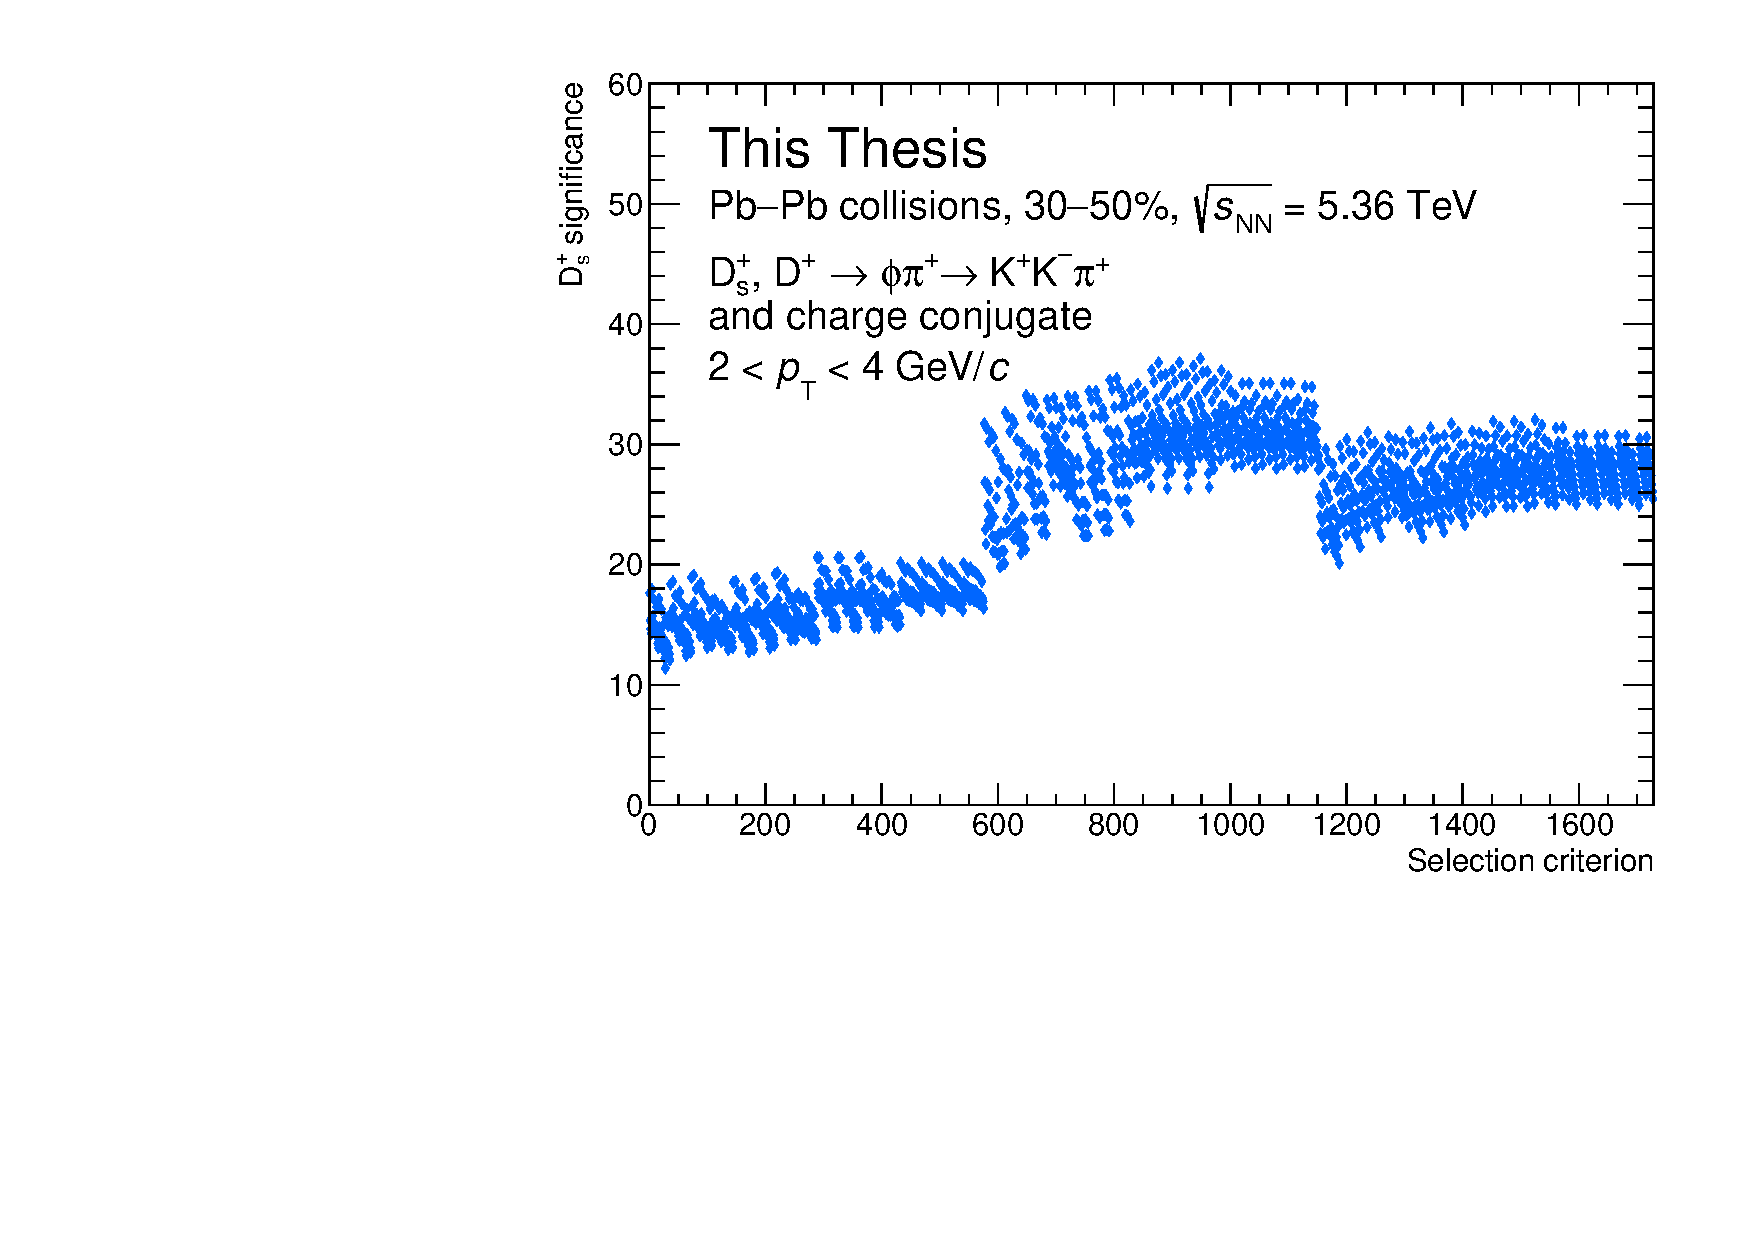
\includegraphics[width=0.7\textwidth]{Figures/Chapter 8/SignificanceScan.pdf}
    \caption{\ds-meson signal statistical significance as a function of the selection criteria for the $2<\pt<4$~\gevc interval in the 30--50\% centrality class.}
    \label{fig:signif_scan_pbpb}
\end{figure}

The optimal selection criteria for the selection of \ds meson candidates in the 10--30\% and 30--50\% centrality classes are reported in the Tables~\ref{tab:optimal_selection_criteria_pbpb_1030} and~\ref{tab:optimal_selection_criteria_pbpb_3050}, respectively. The optimal selection criteria for the 60--90\% centrality class are not reported, as no signal was extracted in this centrality class.

\begin{table}[htb]
    \centering
    \caption{Optimal selection criteria for the selection of \ds meson candidates in the 10--30\% centrality class.}
    \label{tab:optimal_selection_criteria_pbpb_1030}
    \begin{tabular}{l|ccccc}
    \toprule
    & \multicolumn{5}{c}{\pt interval (\gevc)} \\
    Variable & 2$-$4 & 4$-$6 & 6$-$8 & 8$-$12 & 12$-$24 \\
    \midrule
    $L (\si{\micro\meter}) >$ & 600 & 200 & 500 & 200 & 200 \\
    $\cos\theta_\mathrm{p}>$ & 0.99 & 0.998 & 0.9985 & 0.98 & 0.98 \\
    $\cos\theta_\mathrm{p}^{xy}>$ & 0.999 & 0.998 & 0.998 & 0.99 & 0.995 \\
    $\lvert\Delta M(\mathrm{KK})\rvert (\mevcc) <$ & 7 & 9 & 5 & 7 & 7 \\
    $\lvert\cos^3\left(\theta'(\mathrm K)\right)\rvert >$ & 0.3 & 0.2 & 0.2 & 0.2 & 0.3 \\
    $\chi^2_\mathrm{PCA} <$ & 3.0 & 6.0 & 3.0 & 3.0 & 9.0 \\
    \bottomrule
    \end{tabular}
\end{table}

\begin{table}[htb]
    \centering
    \caption{Optimal selection criteria for the selection of \ds meson candidates in the 30--50\% centrality class.}
    \label{tab:optimal_selection_criteria_pbpb_3050}
    \begin{tabular}{l|ccccc}
    \toprule
    & \multicolumn{5}{c}{\pt interval (\gevc)} \\
    Variable & 2$-$4 & 4$-$6 & 6$-$8 & 8$-$12 & 12$-$24 \\
    \midrule
    $L (\si{\micro\meter}) >$ & 400 & 200 & 200 & 200 & 200 \\
    $\cos\theta_\mathrm{p}>$ & 0.996 & 0.998 & 0.998 & 0.98 & 0.995 \\
    $\cos\theta_\mathrm{p}^{xy}>$ & 0.996 & 0.997 & 0.998 & 0.985 & 0.98 \\
    $\lvert\Delta M(\mathrm{KK})\rvert (\mevcc) <$ & 7 & 9 & 9 & 5 & 5 \\
    $\lvert\cos^3\left(\theta'(\mathrm K)\right)\rvert >$ & 0.1 & 0.1 & 0.1 & 0.1 & 0.2 \\
    $\chi^2_\mathrm{PCA} <$ & 3.0 & 3.0 & 12.0 & 12.0 & 9.0 \\
    \bottomrule
    \end{tabular}
\end{table}

\section{Signal extraction}
Once the selection criteria are optimised for each \pt interval and centrality class, the signal is extracted by fitting the invariant mass distribution of the selected candidates. The fit function is composed of an exponential function for describing the background shape and two Gaussian functions for the \ds and \dpl signal peaks. The fit of the invariant mass distributions of the candidates passing the selection criteria described above is performed in the invariant mass range of $1.7 < M < 2.1$~\gevcc. A clear signal peak is observed in both the 10--30\% and 30--50\% centrality classes, with statistical significances ranging from 14 to 35 for \ds mesons and from 4 to 14 for \dpl mesons depending on \pt in the 10--30\% centrality interval, and from 9 to 37 for \ds mesons and from 4 to 21 for \dpl mesons in the 30--50\% centrality class. Figure~\ref{fig:inv_mass_fit_pbpb} shows the normalised invariant mass distribution of D-meson candidates passing the applied selections in the $2<\pt<4$~\gevc (top-left panel) and $6<\pt<8$~\gevc (bottom-left panel) intervals of the 10--30\% centrality class and in the $4<\pt<6$~\gevc (top-right panel) and $8<\pt<12$~\gevc (bottom-right panel) intervals of the 30--50\% centrality class. 

\begin{figure}[htbp]
    \centering
    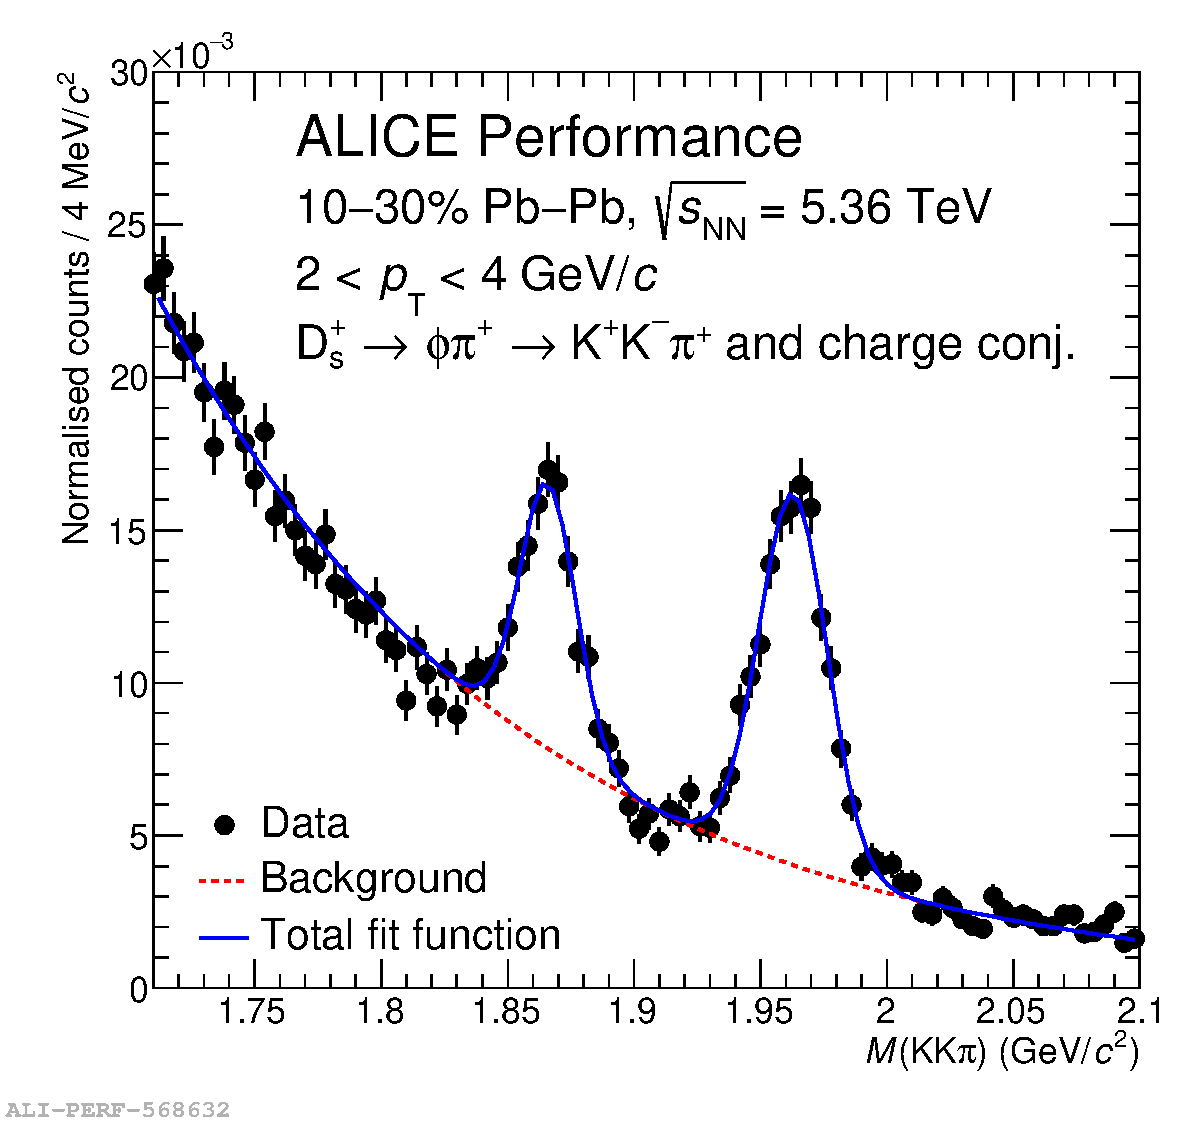
\includegraphics[width=0.48\textwidth]{Figures/Chapter 8/ds_massfit_norm_1030.pdf}
    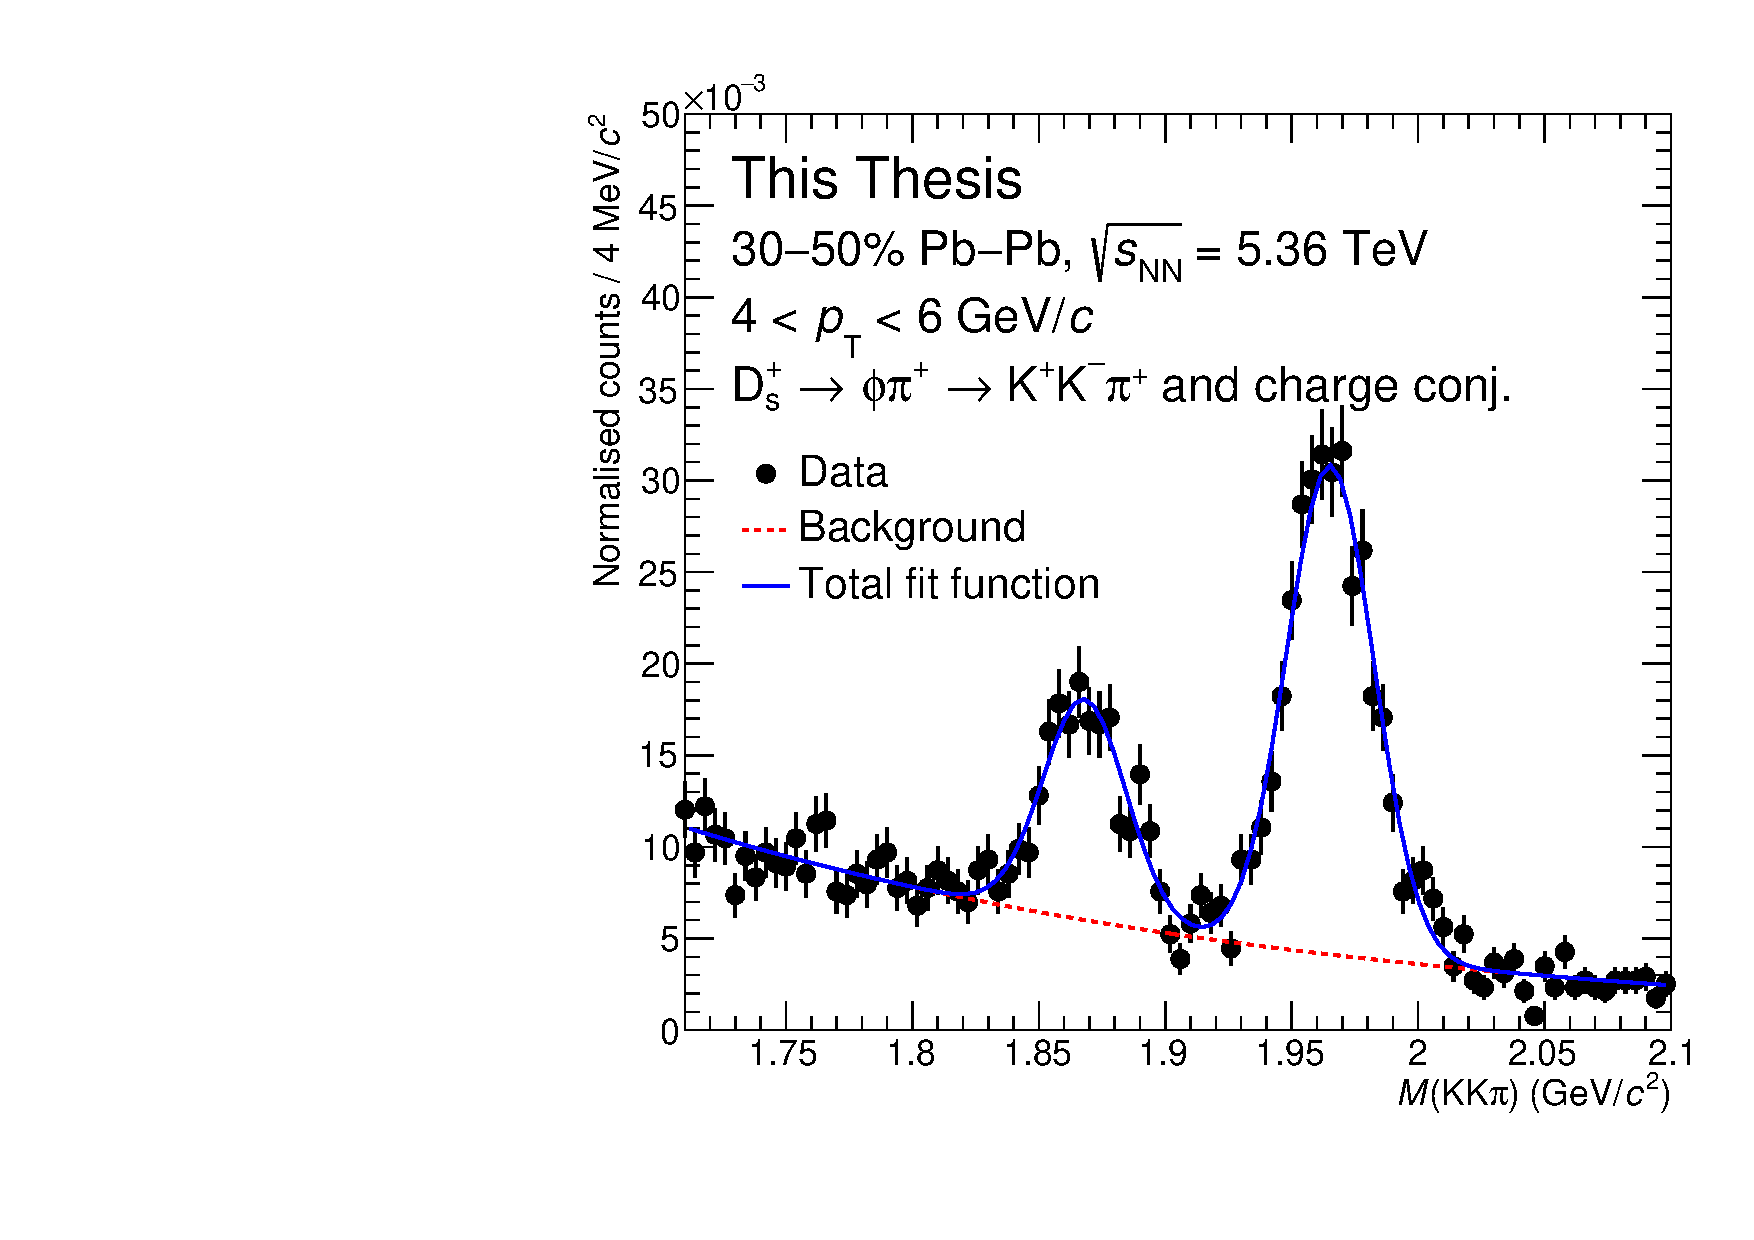
\includegraphics[width=0.48\textwidth]{Figures/Chapter 8/ds_massfit_norm_3050.pdf}
    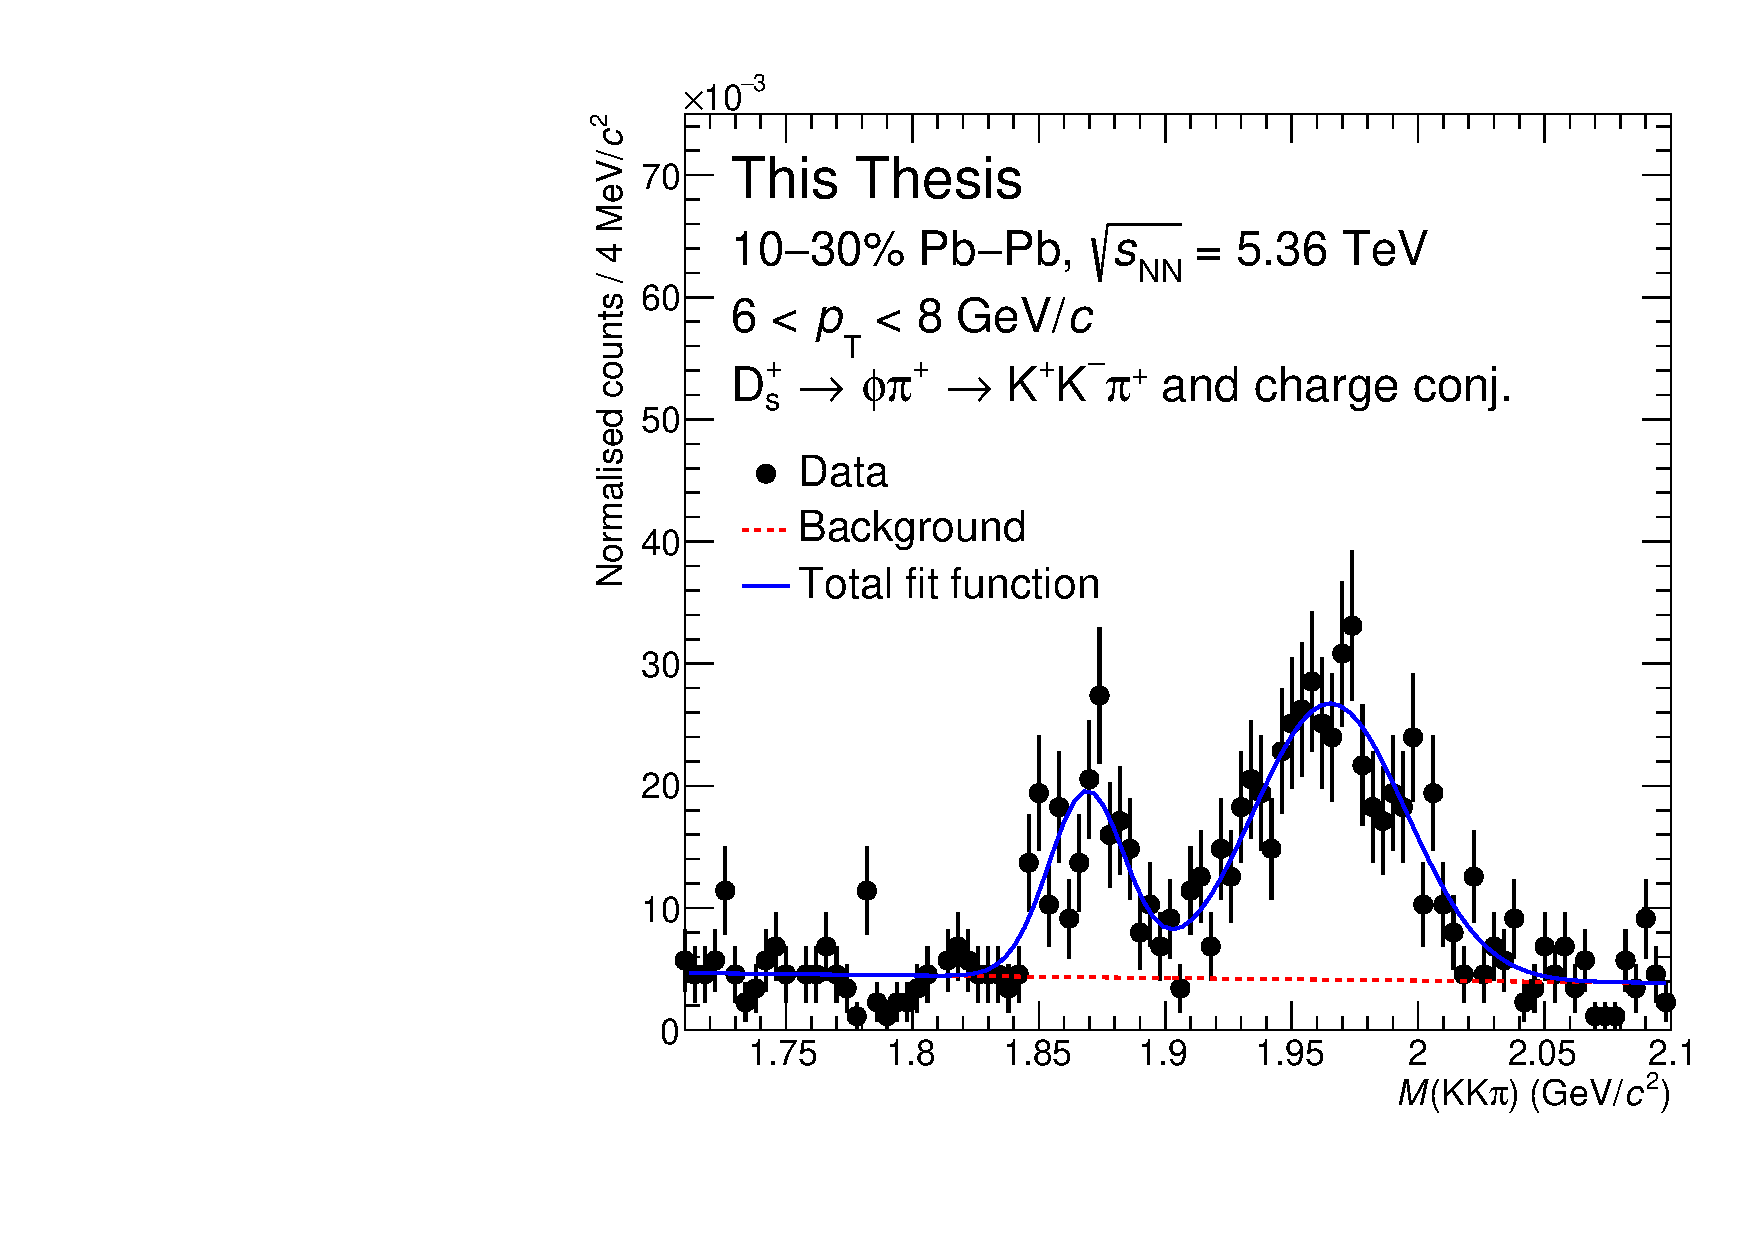
\includegraphics[width=0.48\textwidth]{Figures/Chapter 8/ds_massfit_norm_10_30_6_8.pdf}
    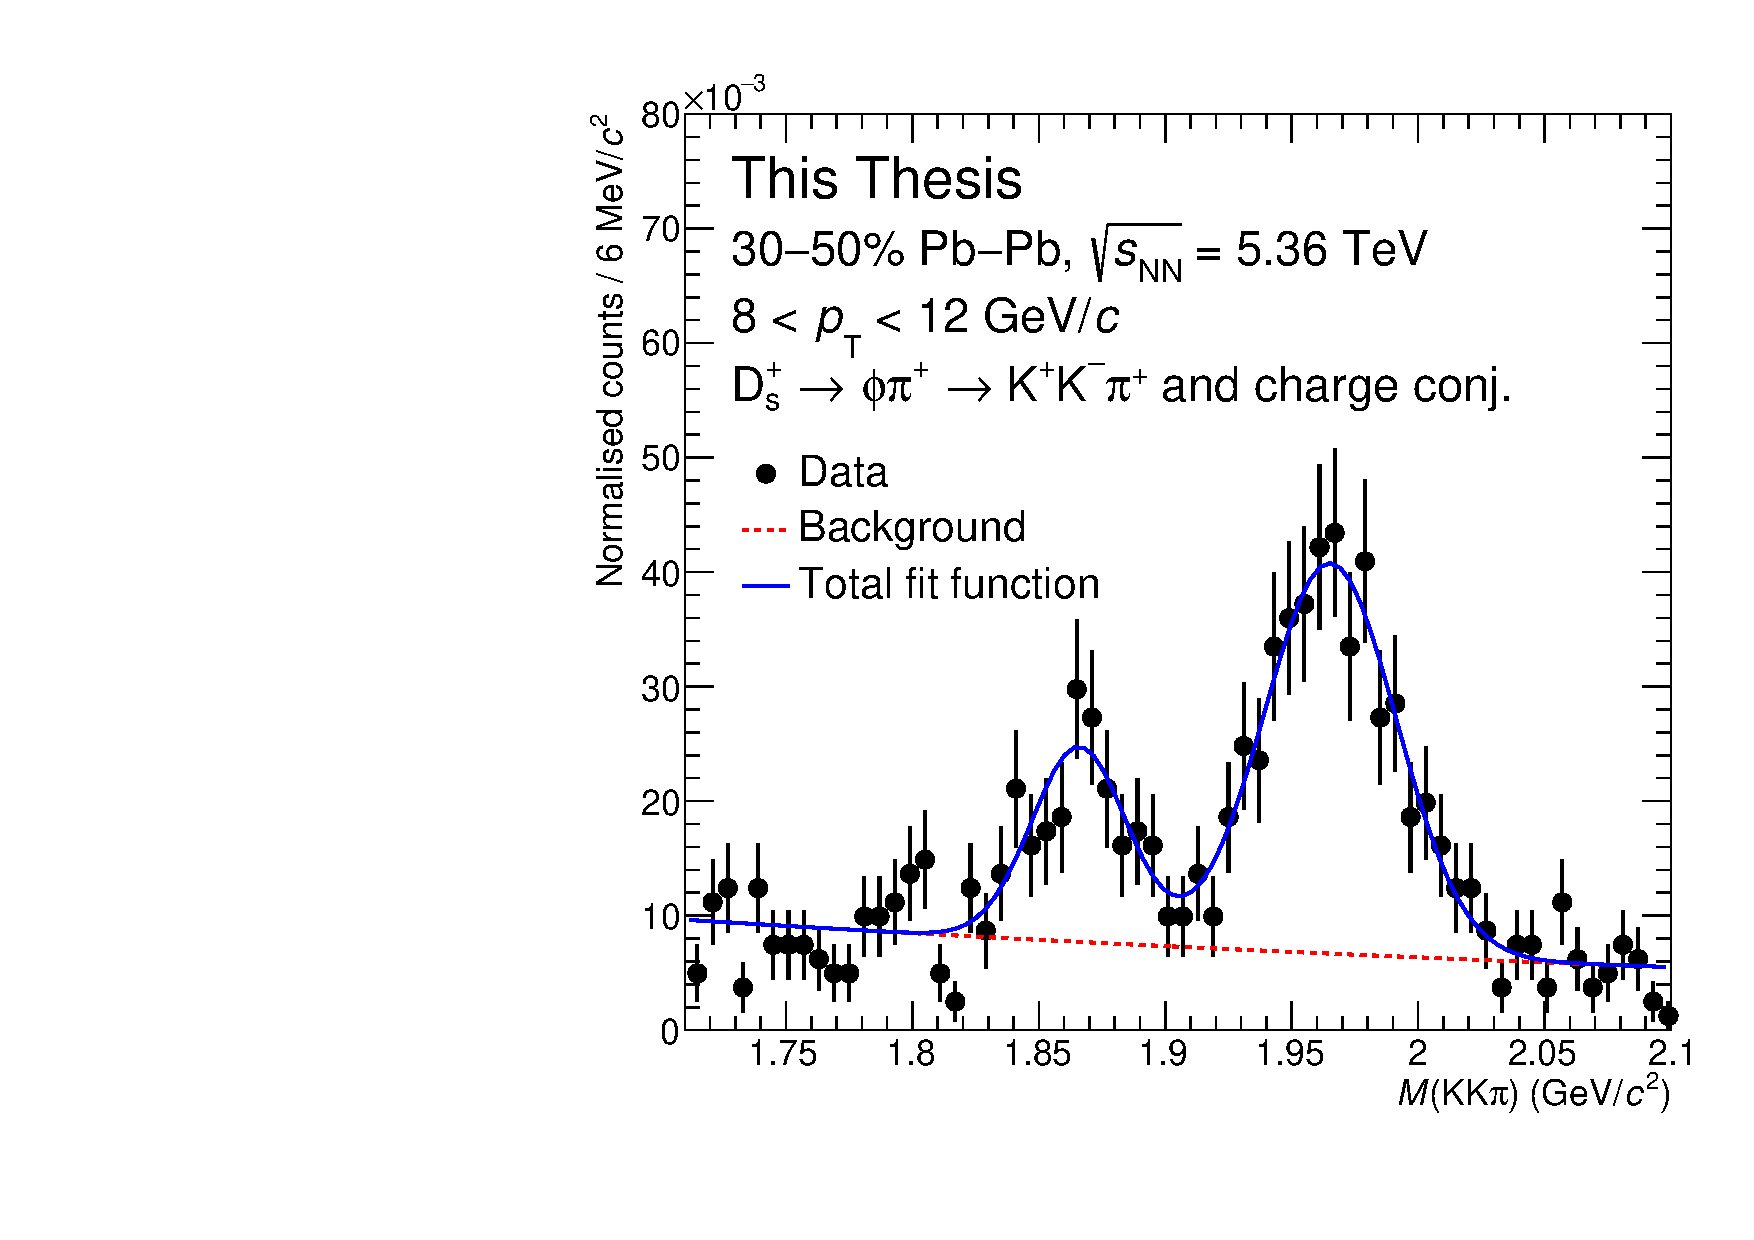
\includegraphics[width=0.48\textwidth]{Figures/Chapter 8/ds_massfit_norm_3050_8_12.pdf}
    \caption{Normalised invariant mass distribution of the selected D-meson candidates in the $2<\pt<4$~\gevc (top-left panel) and $6<\pt<8$~\gevc (bottom-left panel) intervals of the 10--30\% centrality class and in the $4<\pt<6$~\gevc (top-right panel) and $8<\pt<12$~\gevc (bottom-right panel) intervals of the 30--50\% centrality class.}
    \label{fig:inv_mass_fit_pbpb}
\end{figure}

As mentioned above, one of the consequences of the backflow of ions in the TPC is the distortion of the drift paths of the ionised electrons, which leads to a worsening of the track momentum resolution. An increase of the peak widths with increasing \pt is already visible in Fig.~\ref{fig:inv_mass_fit_pbpb}: while the \ds and \dpl peaks are well separated in both the $2<\pt<4$~\gevc and $4<\pt<6$~\gevc intervals, at the higher \pt intervals of $6<\pt<8$~\gevc and $8<\pt<12$~\gevc the peak widths are larger, and the two peaks are partially overlapping. Nevertheless, a worsening in the resolution with increasing \pt is expected due to the reduced track curvature in the presence of the magnetic field. Therefore, to test the validity of the distortion corrections in the reconstruction framework it is useful to study the resolution of the \ds and \dpl mesons peaks, and compare it with that obtained during the LHC Run~2 data-taking period, where fewer distortions were present thanks to the reduced interaction rate and the active ion gates. Similar studies are being performed for the $\mathrm{K^0_s}\rightarrow\pi^+\pi^-$ peaks. However, the measurement of D meson widths allows the test of a different \pt range of the tracks and the effects on the charged kaon reconstruction, which is not possible with the $\mathrm{K^0_s}$ mesons.  

The resolution of the \ds and \dpl mesons peaks is extracted from the fits of the invariant mass distribution of the selected candidates as the standard deviation of the Gaussian function used to describe the D-meson signals. In Figure~\ref{fig:inv_mass_fit_res_pbpb}, the peak width of the \ds meson signal is shown for the analysis performed in this Thesis using the 30--50\% centrality class of Pb--Pb collisions recorded in the LHC Run~3 data-taking period (blue markers) as a function of \pt. A clear increasing trend of the peak width with \pt is observed, and is attributed to the worsening of the momentum resolution with increasing \pt due to the smaller curvature of high-momentum tracks. The peak widths of the \ds-meson signals extracted from the Pb--Pb collisions data collected during the LHC Run~2 data-taking period at $\snn=5.02$~\tev in the 30--50\% centrality class~\cite{ALICE:2021kfc} (shown as green markers in Fig.~\ref{fig:inv_mass_fit_res_pbpb}) are smaller than those foun for Run~3 samples. This is due to the distortions of the electric field in the TPC, which were smaller in Run~2 because the TPC ion backflow was significantly suppressed using active gating grids. Lastly, the peak widths of the \ds-meson signals extracted from pp collisions data recorded during the LHC Run~3 data-taking period at \thirteen in this Thesis (as described in Chapter~\ref{chap:RY}) are reported as a function of \pt with red markers. These results show a magnitude of the width and a trend with \pt which are consistent with what is observed in Pb--Pb collisions at \fivenn, confirming that the observed worsening of the momentum resolution is due to the backflow of ions in the TPC, which affect similarly the different samples of pp and Pb--Pb collisions collected during the LHC Run~3 data-taking period. The widths extracted in pp collisions are systematically smaller than those from Pb--Pb collisions, albeit being compatible within uncertainties. This effect may be due to a newer reconstruction performed in the pp collisions data, which may have improved the momentum resolution. Studies are currently ongoing to further improve the calibration of the reconstruction and improve the momentum resolution in both pp and Pb--Pb collisions, allowing for more precise measurements of the production of D mesons. 

\begin{figure}
    \centering
    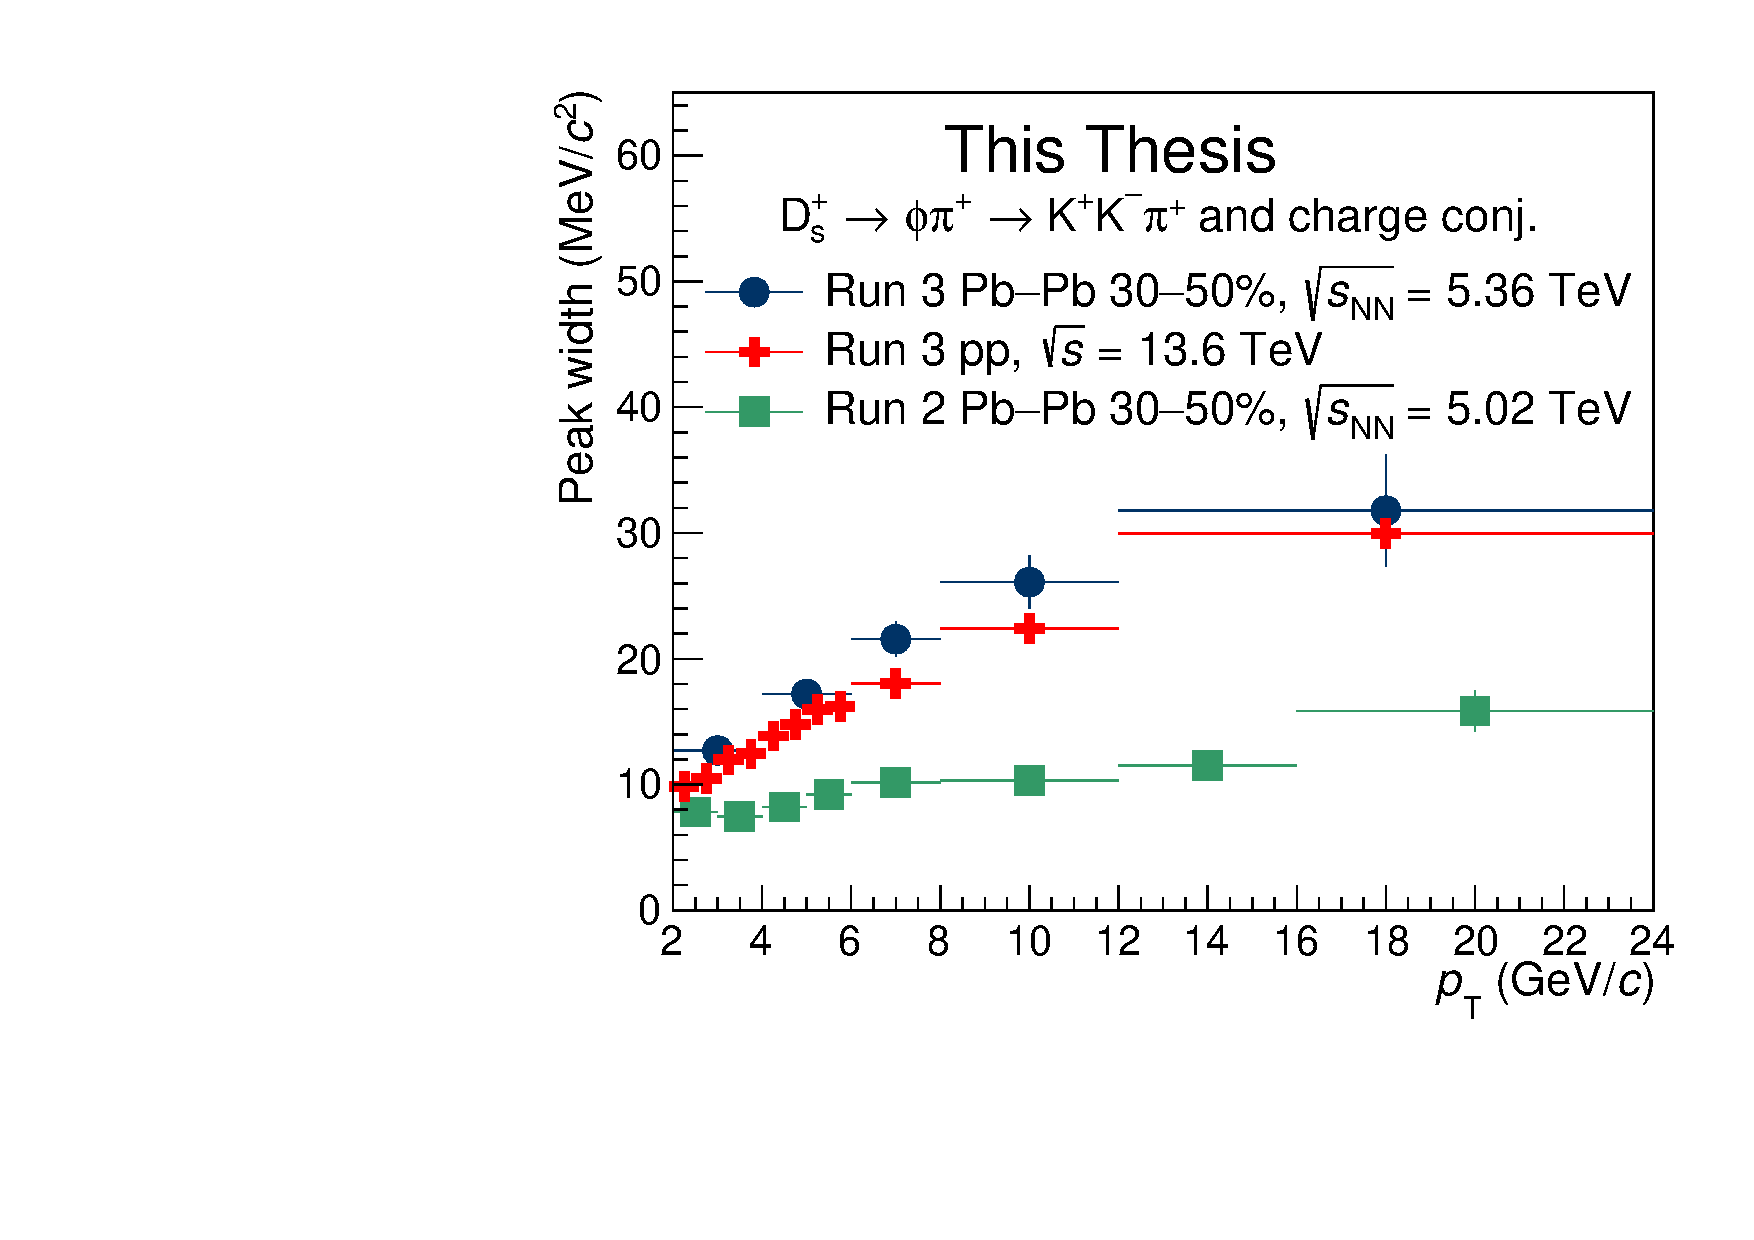
\includegraphics[width=0.7\textwidth]{Figures/Chapter 8/Ds_widths_performance.pdf}
    \caption{Width of the \ds-meson signal peak as a function of \pt measured in Pb--Pb collisions at \fivenn in the 30--50\% centrality class and pp collisions at \thirteen recorded during the LHC Run~3 data-taking period  (blue and red markers, respectively) and in the 30--50\% centrality class of Pb--Pb collisions at $\snn=5.02$~\tev recorded during the LHC Run~2 data-taking period (green markers).}
    \label{fig:inv_mass_fit_res_pbpb}
\end{figure}
